\documentclass{article}
\usepackage{graphicx} % Required for inserting images
\usepackage{varwidth}

\title{Experiment 1 Lab Report \\ \large EEE3342C - 00012}
\author{Yousef Awad}
\date{January 2025}
\setcounter{secnumdepth}{0}

\begin{document}

\maketitle
\tableofcontents
\newpage

\section{Equipment}
\qquad
For this experiment a Windows 11 computer was used alongside the Xilinx Vivado 2024.2 software, alongside an FPGA board, the BASYS 3 development board. The board specifically only used to ensure the simulation by the Vivado software was accurate in the real world.\\
\section{Objective}
\qquad
The objective that was given in the experiment was to introduce the Vivado software as well as the following binary operators: AND, OR, XOR, and the unary operator of the Inverter. Alongside this two circuits were made, one with 2 inputs (of which variations for all the binary operators were made) as well as with 5 inputs (of which all the operators were used). They were then simulated, as well as pushed to the FPGA board for testing and confirmation respectively.\\
\section{Design Steps (General/Part 1)}
\qquad
To begin with all of the schematics (listed below in Section 4), I first had to create a project via opening the Vivado software. After opening the software I then went to the top left of the screen, under the "File" tab and then clicked on "Project" and then "New" (as shown on Figure 1).\\
\begin{figure}[!htbp]
    \centering
    \caption{}
    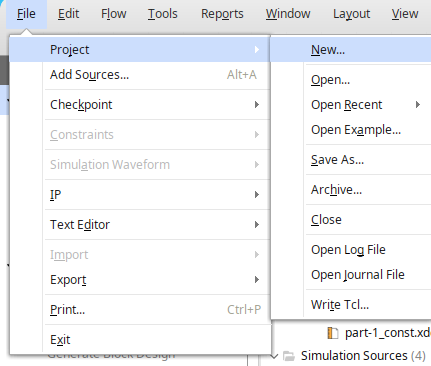
\includegraphics[width=0.5\textwidth]{figure_3_1.png}
    \label{Figure 3.1}
\end{figure}\newline
After clicking on "New", I then went through the prompts, defining the name of the project (for example "Experiment-1"), as well as its location (for example "C:/user/yousef/Desktop/experiment-1/"). After this I selected the type of project that I am creating a "RTL Project" of which is a full circuit design alongside its constraints as well as allows for simulation. After this, I then create a "source file", which is a Verilog file (ending with .v) that defines the inputs and outputs of a circuit, alongside what it does specifically (See figure 2 for specifics).\\
\begin{figure}[!htbp]
    \centering
    \caption{}
    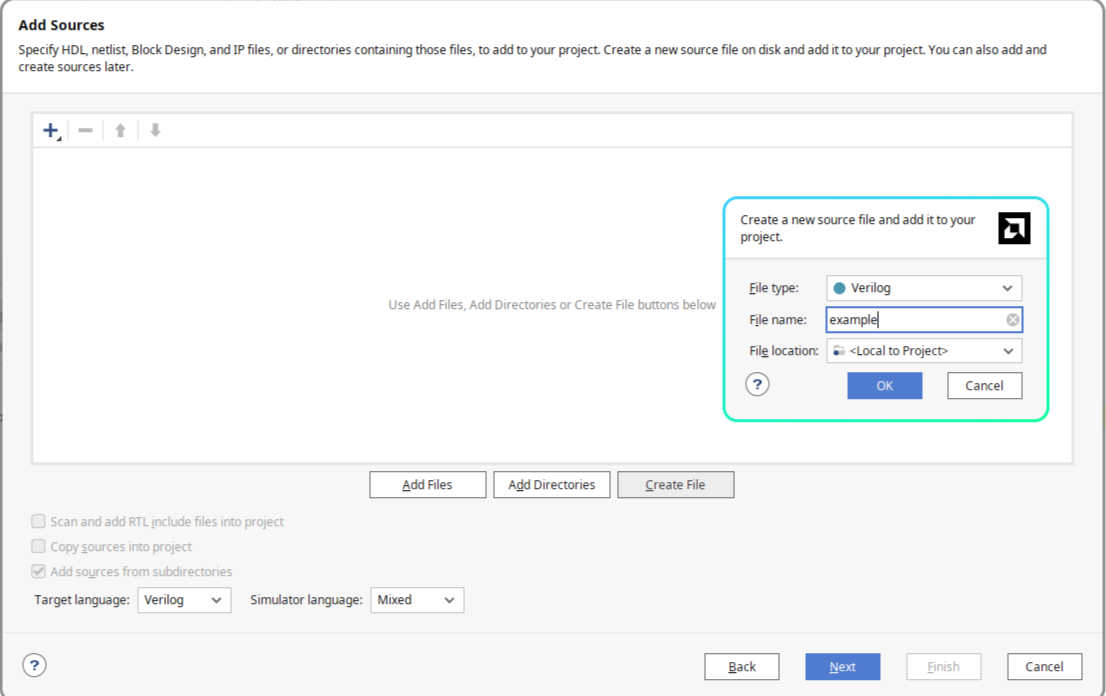
\includegraphics[width=0.5\textwidth]{figure_3_2.png}
    \label{Figure 3.2}
\end{figure}\newline
After this I then ignored the rest of the prompts and opened the Verilog file I created during the setup. What opened up for me then, was the project summary screen (example shown in Figure 3), with to the left of it being the Sources window showing the "Design Sources" (where we design the circuit), the "Constraints" (where we define the ports on the FPGA as well as how it should actually simulate it), as well as the "Simulation Sources" (which let's us create a test-bench to test the circuit we made in the Design Sources).\\
\begin{figure}[!htbp]
    \centering
    \caption{}
    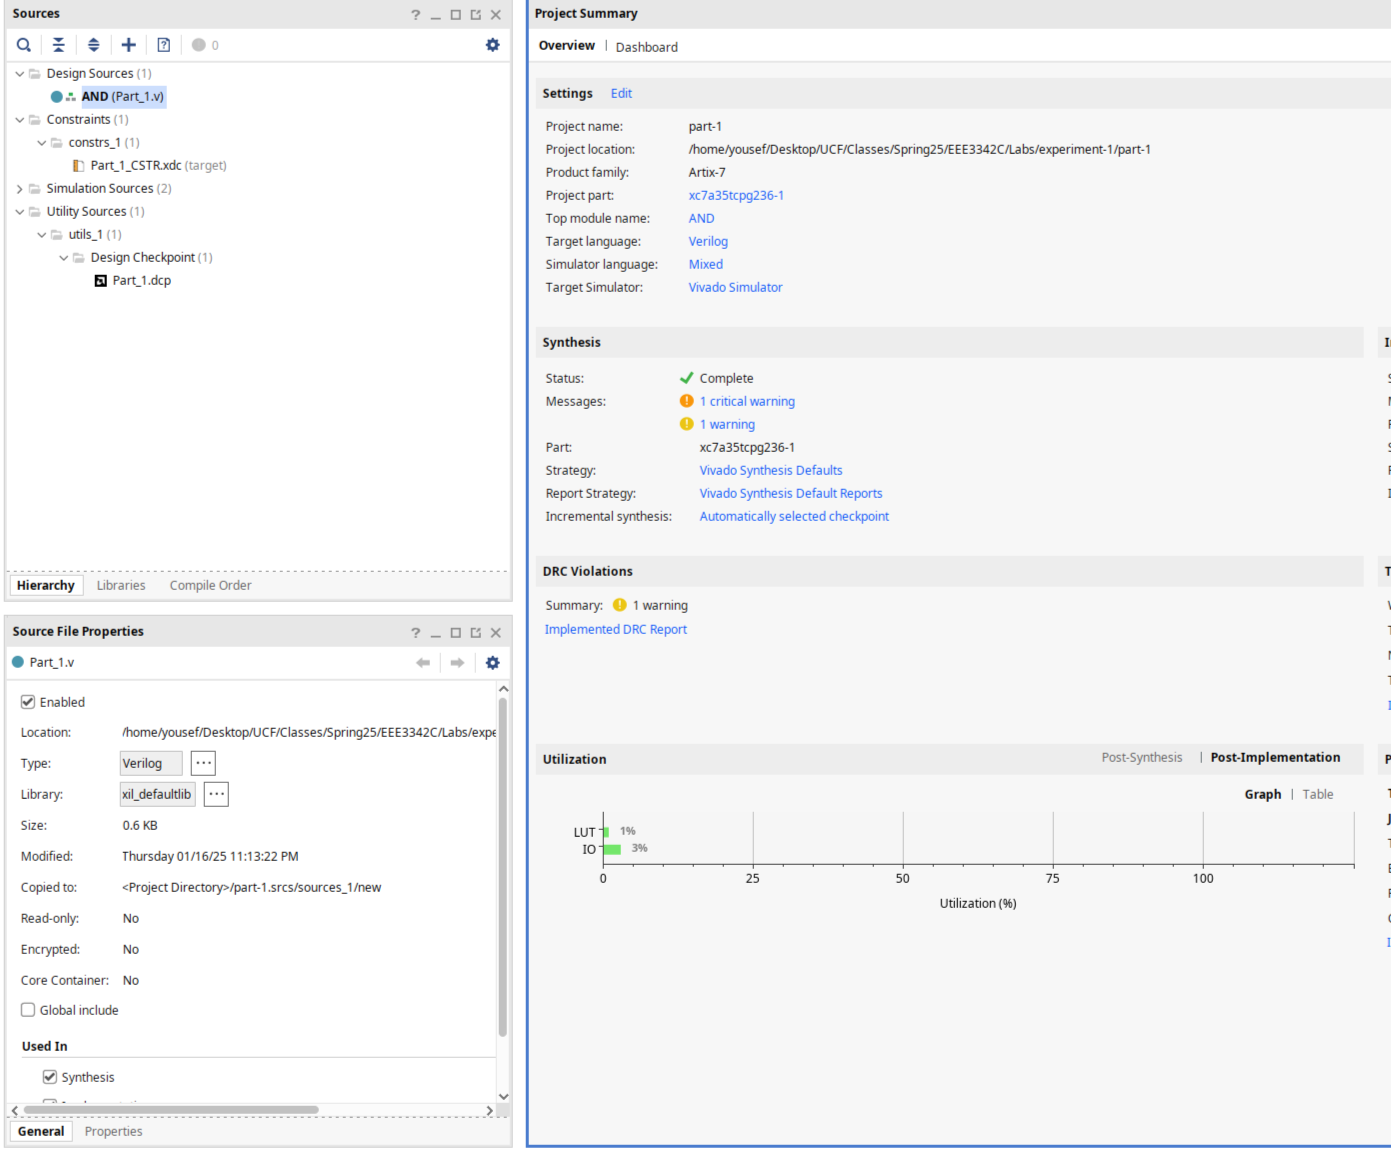
\includegraphics[width=0.5\textwidth]{figure_3_3.png}
    \label{Figure 3.3}
\end{figure}
\newpage
\section{Design Steps (Specific)}
\subsection{AND Gate}
After this, I then began to create an AND gate, of which looks like the following, at its most basic form:
\begin{figure}[!htbp]
    \centering
    \caption{AND Gate}
    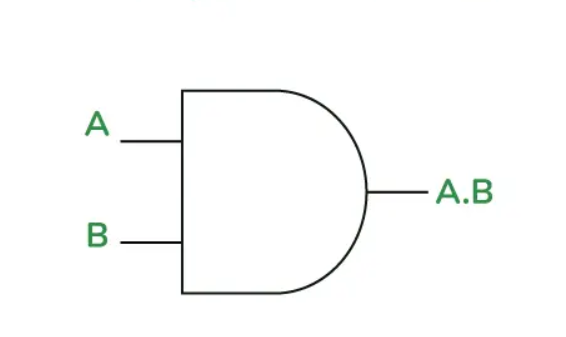
\includegraphics[width=0.5\textwidth]{AND-GATE.png}
    \label{AND Gate, Simple}
\end{figure}\\
After inputting the following code for the Verilog module, of which is shown below in Figure 5, I then compiled the schematic to ensure that it is correctly modeled.
\begin{figure}[!htbp]
    \centering
    \caption{Verilog Code for AND Gate}
    \begin{verbatim}
    module AND(
        input In1, In2,
        output Out
        );
        
        assign Out = In1 & In2;
        
    endmodule
    \end{verbatim}
\end{figure}\newline
And from that code it compiled this schematic (Figure 6) which has 2 inputs, being A and B, as well as one output, being Out. Alongside this, the device floor plan is shown as well, in Figure 7, as properly implemented according to the basic form shown in Figure 4, as well as the constraints for the simulation to take place (shown in Figure 8).
\begin{figure}[!htbp]
    \centering
    \caption{AND Gate Schematic}
    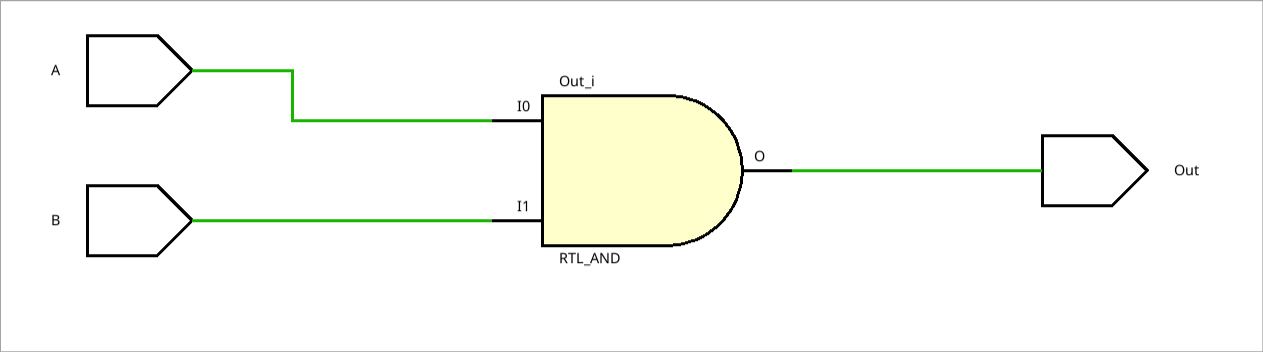
\includegraphics[width=0.5\textwidth]{AND-GATE-SCHEMATIC.png}
    \label{AND Gate, Schematic}
\end{figure}
\begin{figure}[!htbp]
    \centering
    \caption{AND Gate Floor Plan}
    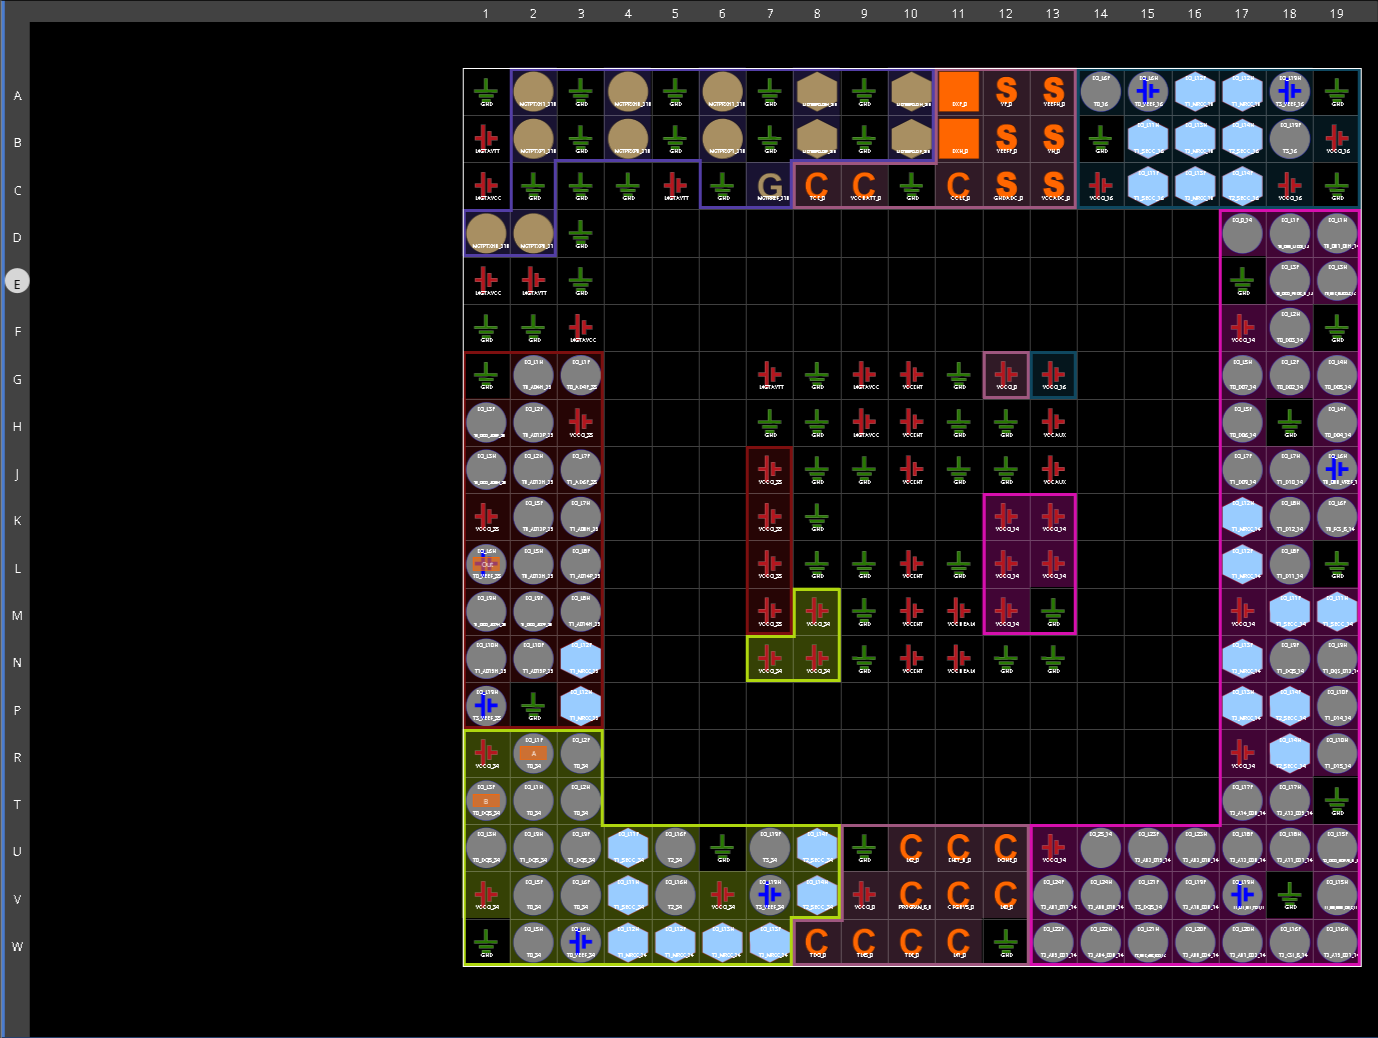
\includegraphics[width=0.5\textwidth]{AND-GATE-FLOOR-PLAN.png}
    \label{AND Gate, Floor Plan}
\end{figure}
\begin{figure}[!htbp]
    \centering
    \caption{AND Gate Constraints}
    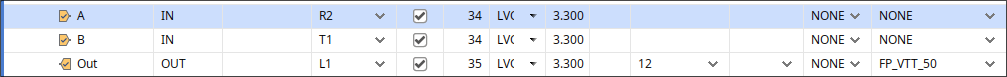
\includegraphics[width=0.75\textwidth]{AND-GATE-CONSTRAINTS.png}
    \label{AND Gate, Constrants}
\end{figure}\newpage
After this, I then ran the waveform simulation properly, as the circuit was properly implemented, as well as having the correct schematic. The waveform returned the following, as shown in Figure 9, as well as shown in Table 1 with its truth table.
\begin{figure}[!htbp]
    \centering
    \caption{AND Gate Waveform}
    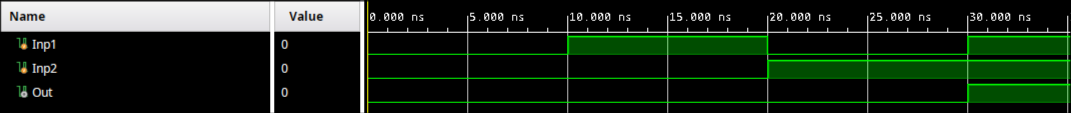
\includegraphics[width=0.75\textwidth]{AND-GATE-WAVEFORM.png}
    \label{AND Gate, Waveform}
\end{figure}\newline
\begin{center}
    Truth Table 1: AND Gate Waveform
    \begin{displaymath}
    \begin{array}{|c c|c|}
    In1 & In2 & In1 \land In2\\
    \hline
    F & F & F\\
    F & T & F\\
    T & F & F\\
    T & T & T\\
    \end{array}
    \end{displaymath}
\end{center}
Now, for context, all the waveform is explaining to us is that, as expected, when both of the Inputs are true, the output shall be true, otherwise the output is false.
\newpage
\subsection{NAND Gate}
Now to create an NAND gate, of which looks like the following, at its most basic form:
\begin{figure}[!htbp]
    \centering
    \caption{NAND Gate}
    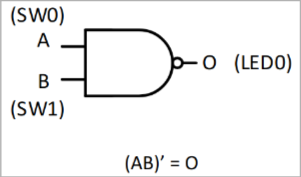
\includegraphics[width=0.5\textwidth]{NAND-GATE.png}
    \label{NAND Gate, Simple}
\end{figure}\newline
After inputting the following code for the Verilog module, of which is shown below in Figure 11, I then compiled the schematic to ensure that it is correctly modeled.
\begin{figure}[!htbp]
    \centering
    \caption{Verilog Code for NAND Gate}
    \begin{verbatim}
    module NAND(
        input A, B,
        output Out
        );
        
        assign Out = ~(A & B);
        
    endmodule
    \end{verbatim}
\end{figure}\\
And from that code it compiled this schematic (Figure 12) which has 2 inputs, being A and B, as well as one output, being Out. Alongside this, the device floor plan is shown as well, in Figure 13, as properly implemented according to the basic form shown in Figure 10, as well as the constraints for the simulation to take place (shown in Figure 14).
\begin{figure}[!htbp]
    \centering
    \caption{NAND Gate Schematic}
    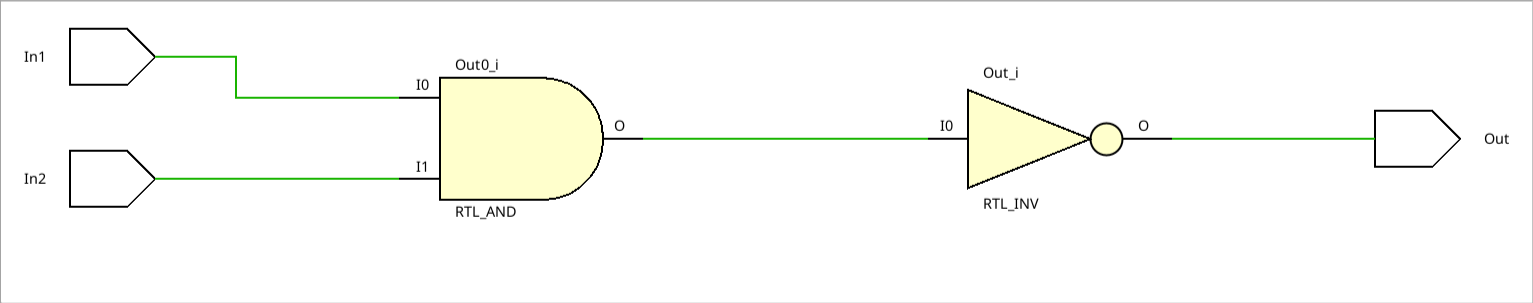
\includegraphics[width=0.5\textwidth]{NAND-GATE-SCHEMATIC.png}
    \label{NAND Gate, Schematic}
\end{figure}
\begin{figure}[!htbp]
    \centering
    \caption{NAND Gate Floor Plan}
    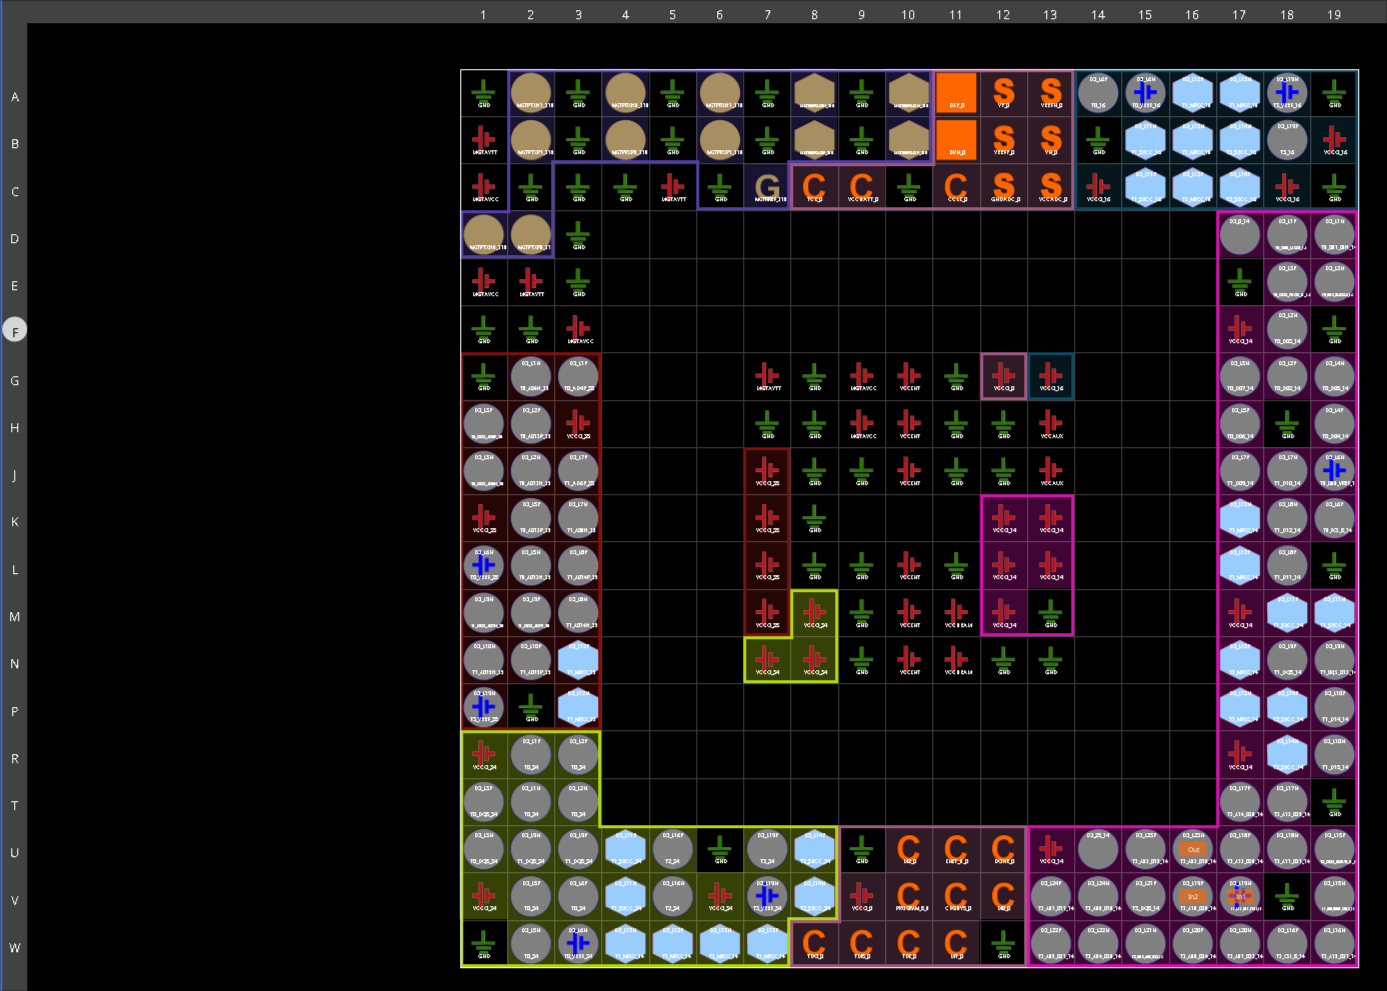
\includegraphics[width=0.5\textwidth]{NAND-GATE-FLOOR-PLAN.png}
    \label{NAND Gate, Floor Plan}
\end{figure}
\begin{figure}[!htbp]
    \centering
    \caption{NAND Gate Constraints}
    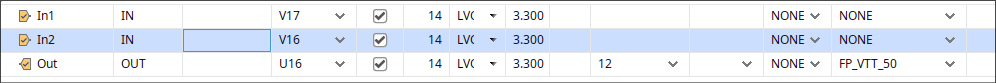
\includegraphics[width=0.75\textwidth]{NAND-GATE-CONSTRAINTS.png}
    \label{NAND Gate, Constrants}
\end{figure}\newpage
After this, I then ran the waveform simulation properly, as the circuit was properly implemented, as well as having the correct schematic. The waveform returned the following, as shown in Figure 15, as well as shown in Table 2 with its truth table.
\begin{figure}[!htbp]
    \centering
    \caption{NAND Gate Waveform}
    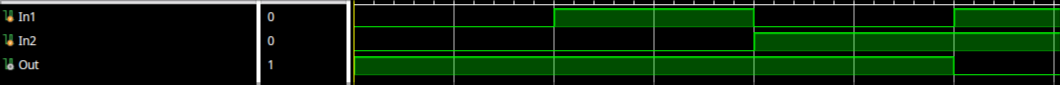
\includegraphics[width=0.75\textwidth]{NAND-GATE-WAVEFORM.png}
    \label{NAND Gate, Waveform}
\end{figure}\\
\begin{center}
    Truth Table 2: NAND Gate Waveform
    \begin{displaymath}
    \begin{array}{|c c|c|}
    In1 & In2 & \neg(In1 \land In2)\\
    \hline
    F & F & T\\
    F & T & T\\
    T & F & T\\
    T & T & F\\
    \end{array}
    \end{displaymath}
\end{center}
Now, to explain the waveform, all it is showing is that when both inputs are not enabled, or true as shown in the truth table, the output result shall be true/enabled.
\newpage
\subsection{OR Gate}
Now to create an OR gate, of which looks like the below figure, at its most basic form.\\
\begin{figure}[!htbp]
    \centering
    \caption{OR Gate}
    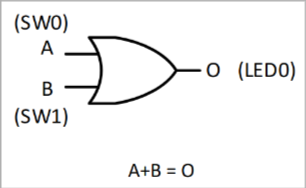
\includegraphics[width=0.5\textwidth]{OR-GATE.png}
    \label{OR Gate, Simple}
\end{figure}\\
After inputting the following code for the Verilog module, of which is shown below in Figure 17, I then compiled the schematic to ensure that it is correctly modeled.\\
\begin{figure}[!htbp]
    \centering
    \caption{Verilog Code for OR Gate}
    \begin{verbatim}
    module OR(
        input A, B,
        output Out
        );
        
        assign Out = A | B;
        
    endmodule
    \end{verbatim}
\end{figure}
And from that code it compiled this schematic (Figure 18) which has 2 inputs, being A and B, as well as one output, being Out. Alongside this, the device floor plan is shown as well, in Figure 19, as properly implemented according to the basic form shown in Figure 16, as well as the constraints for the simulation to take place (shown in Figure 20).\\
\begin{figure}[!htbp]
    \centering
    \caption{OR Gate Schematic}
    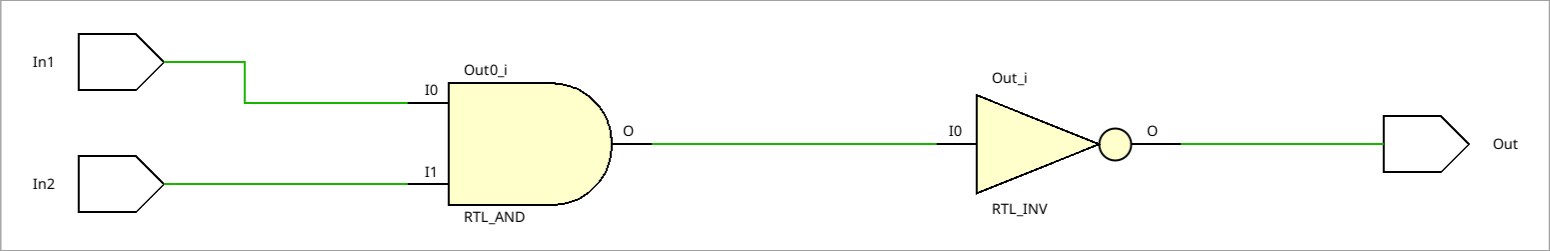
\includegraphics[width=0.5\textwidth]{OR-GATE-SCHEMATIC.png}
    \label{OR Gate, Schematic}
\end{figure}\\
\begin{figure}[!htbp]
    \centering
    \caption{OR Gate Floor Plan}
    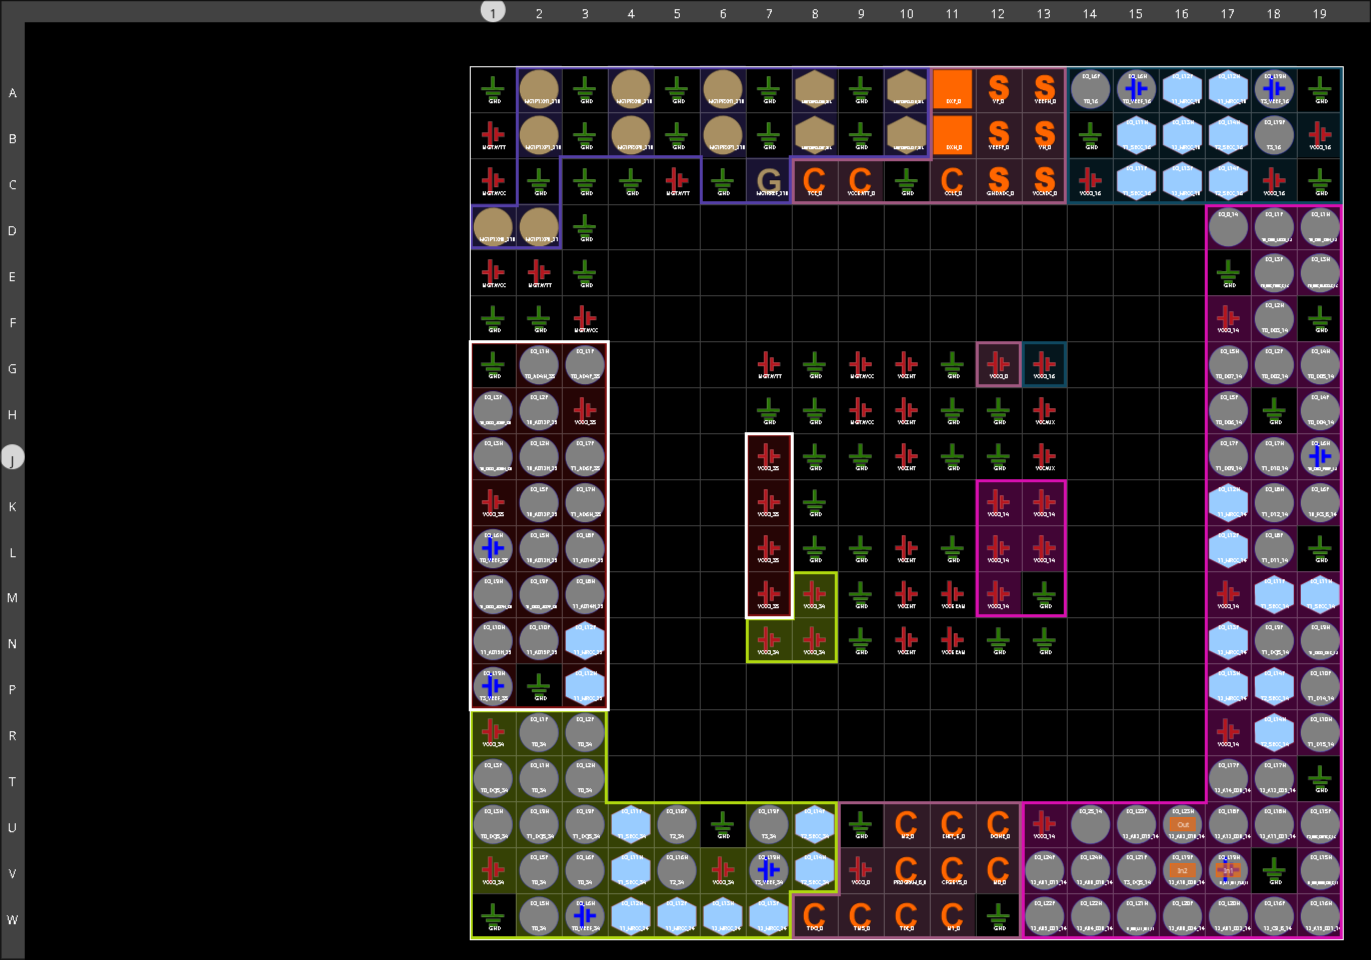
\includegraphics[width=0.5\textwidth]{OR-GATE-FLOOR-PLAN.png}
    \label{OR Gate, Floor Plan}
\end{figure}\\
\begin{figure}[!htbp]
    \centering
    \caption{OR Gate Constraints}
    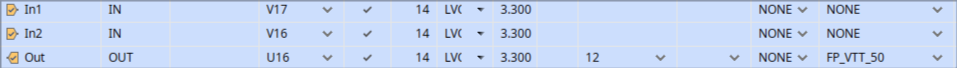
\includegraphics[width=0.75\textwidth]{OR-GATE-CONSTRAINTS.png}
    \label{OR Gate, Constrants}
\end{figure}\\
After this, I then ran the waveform simulation properly, as the circuit was properly implemented, as well as having the correct schematic. The waveform returned the following, as shown in Figure 21, as well as shown in Table 3 with its truth table.\\
\begin{figure}[!htbp]
    \centering
    \caption{OR Gate Waveform}
    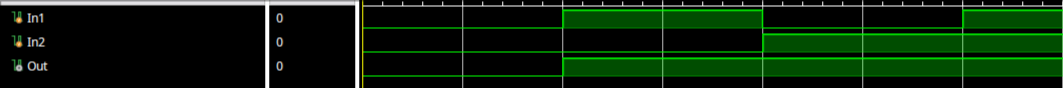
\includegraphics[width=0.75\textwidth]{OR-GATE-WAVEFORM.png}
    \label{OR Gate, Waveform}
\end{figure}\\
\begin{center}
    Truth Table 3: OR Gate Waveform
    \begin{displaymath}
    \begin{array}{|c c|c|}
    In1 & In2 & In1 \lor In2\\
    \hline
    F & F & F\\
    F & T & T\\
    T & F & T\\
    T & T & T\\
    \end{array}
    \end{displaymath}
\end{center}
The waveform, in this case, is specifically showing that, when translated to a proper truth table, the output is On/True only if at least one input is enabled/true.
\newpage
\subsection{XOR Gate}
Now to create an XOR gate, of which looks like the following, at its most basic form.
\begin{figure}[!htbp]
    \centering
    \caption{XOR Gate}
    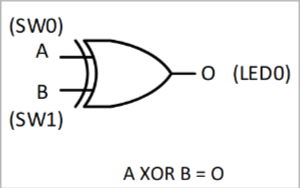
\includegraphics[width=0.5\textwidth]{XOR-GATE.png}
    \label{XOR Gate, Simple}
\end{figure}\\
After inputting the following code for the Verilog module, of which is shown below in Figure 23, I then compiled the schematic to ensure that it is correctly modeled.
\begin{figure}[!htbp]
    \centering
    \caption{Verilog Code for XOR Gate}
    \begin{verbatim}
    module XOR(
        input A, B,
        output Out
        );
        
        assign Out = A ^ B;
        
    endmodule
    \end{verbatim}
\end{figure}\\
And from that code it compiled this schematic (Figure 24) which has 2 inputs, being A and B, as well as one output, being Out. Alongside this, the device floor plan is shown as well, in Figure 25, as properly implemented according to the basic form shown in Figure 22, as well as the constraints for the simulation to take place (shown in Figure 26).
\begin{figure}[!htbp]
    \centering
    \caption{XOR Gate Schematic}
    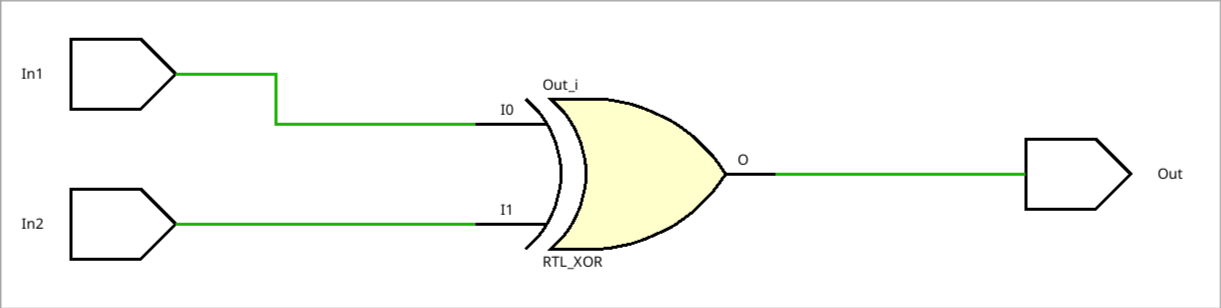
\includegraphics[width=0.5\textwidth]{XOR-GATE-SCHEMATIC.png}
    \label{XOR Gate, Schematic}
\end{figure}
\begin{figure}[!htbp]
    \centering
    \caption{XOR Gate Floor Plan}
    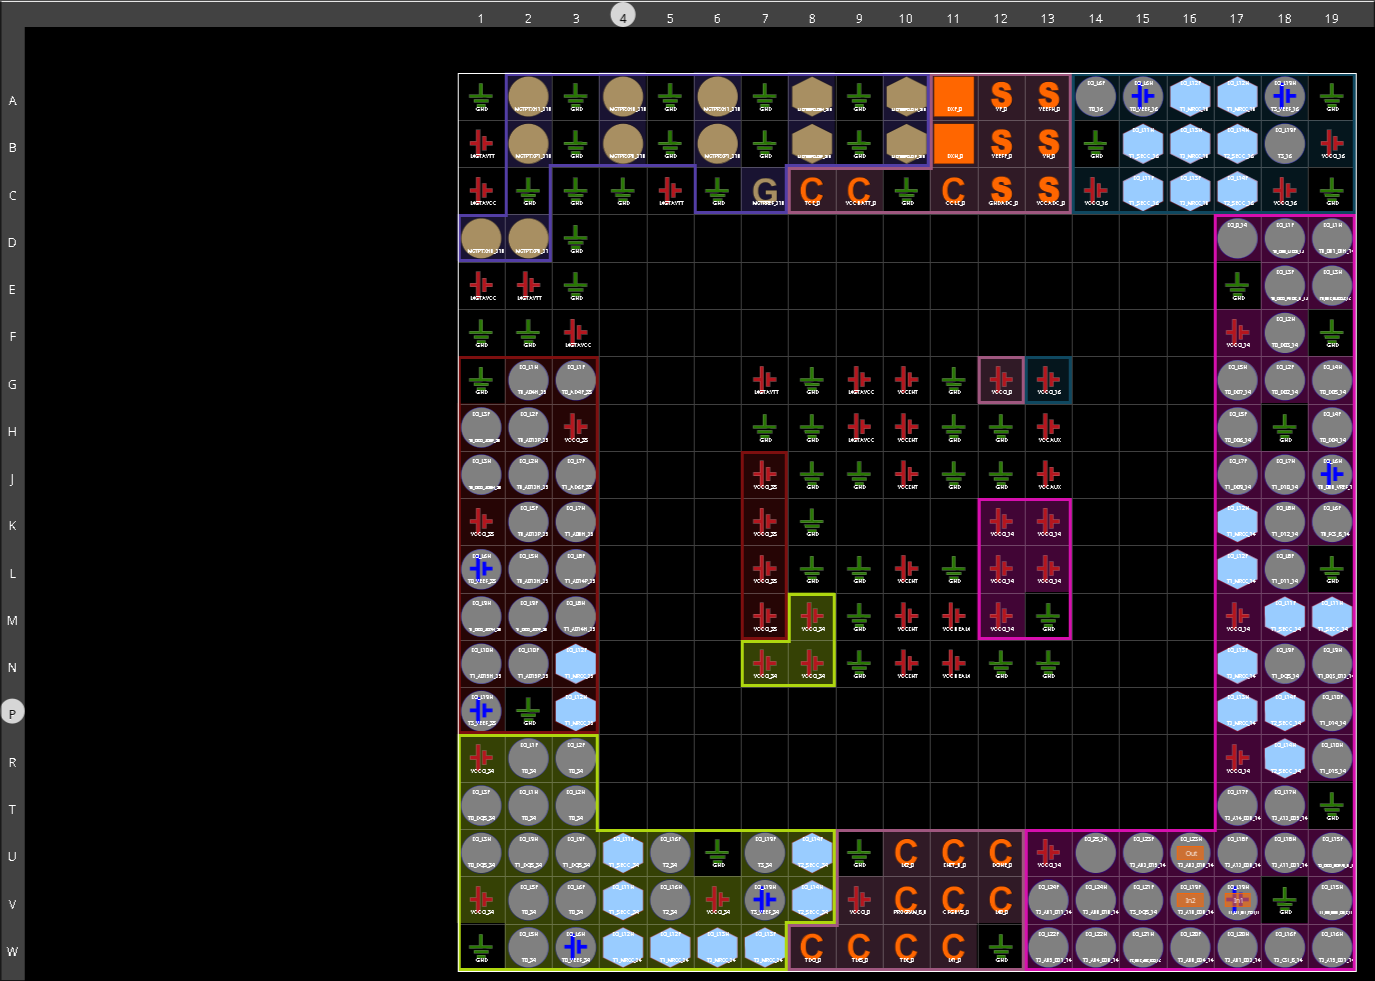
\includegraphics[width=0.5\textwidth]{XOR-GATE-FLOOR-PLAN.png}
    \label{XOR Gate, Floor Plan}
\end{figure}
\begin{figure}[!htbp]
    \centering
    \caption{XOR Gate Constraints}
    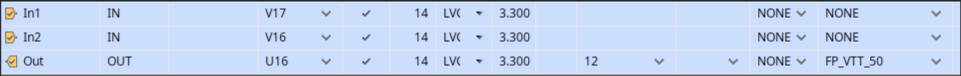
\includegraphics[width=0.75\textwidth]{XOR-GATE-CONSTRAINTS.png}
    \label{XOR Gate, Constrants}
\end{figure}\\
After this, I then ran the waveform simulation properly, as the circuit was properly implemented, as well as having the correct schematic. The waveform returned the following, as shown in Figure 27, as well as shown in Table 4 with its truth table.
\begin{figure}[!htbp]
    \centering
    \caption{XOR Gate Waveform}
    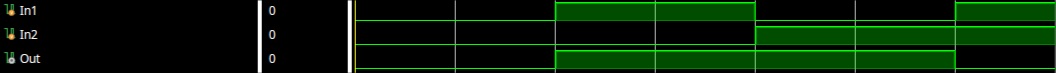
\includegraphics[width=0.75\textwidth]{XOR-GATE-WAVEFORM.png}
    \label{XOR Gate, Waveform}
\end{figure}
\begin{center}
    Truth Table 4: XOR Gate Waveform
    \begin{displaymath}
    \begin{array}{|c c|c|}
    In1 & In2 & In1 \oplus In2\\
    \hline
    F & F & F\\
    F & T & T\\
    T & F & T\\
    T & T & F\\
    \end{array}
    \end{displaymath}
\end{center}
The waveform in this instance shows that the output is only true/enabled only when ONE, not both, input is enabled/true.
\newpage % Inverter Starts Here
\subsection{Inverter Gate}
Now to create an Inverter gate, of which looks like the following, at its most basic form.\\
\begin{figure}[!htbp]
    \centering
    \caption{Inverter Gate}
    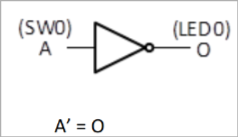
\includegraphics[width=0.5\textwidth]{Inverter-GATE.png}
    \label{Inverter Gate, Simple}
\end{figure}\\
After inputting the following code for the Verilog module, of which is shown below in Figure 29, I then compiled the schematic to ensure that it is correctly modeled.\\
\begin{figure}[!htbp]
    \centering
    \caption{Verilog Code for Inverter Gate}
    \begin{verbatim}
    module INVERTER(
        input A,
        output Out
        );
        
        assign Out = ~A;
        
    endmodule
    \end{verbatim}
\end{figure}\\
And from that code it compiled this schematic (Figure 30) which has 1 input, being A, as well as one output, being Out. Alongside this, the device floor plan is shown as well, in Figure 31, as properly implemented according to the basic form shown in Figure 28, as well as the constraints for the simulation to take place (shown in Figure 32).
\begin{figure}[!!htbpbp]
    \centering
    \caption{Inverter Gate Schematic}
    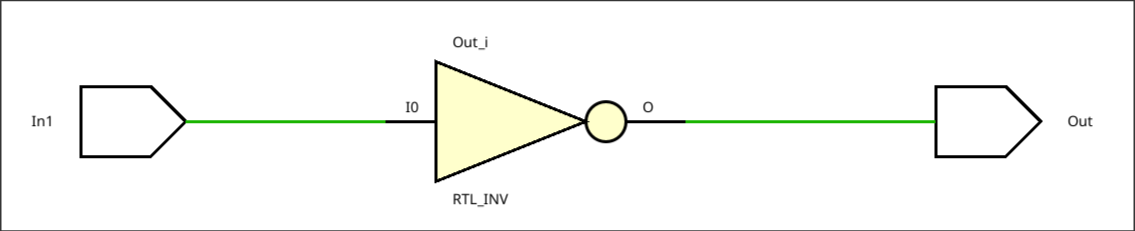
\includegraphics[width=0.5\textwidth]{Inverter-GATE-SCHEMATIC.png}
    \label{Inverter}
\end{figure}
\begin{figure}[!!htbpbp]
    \centering
    \caption{Inverter Gate Floor Plan}
    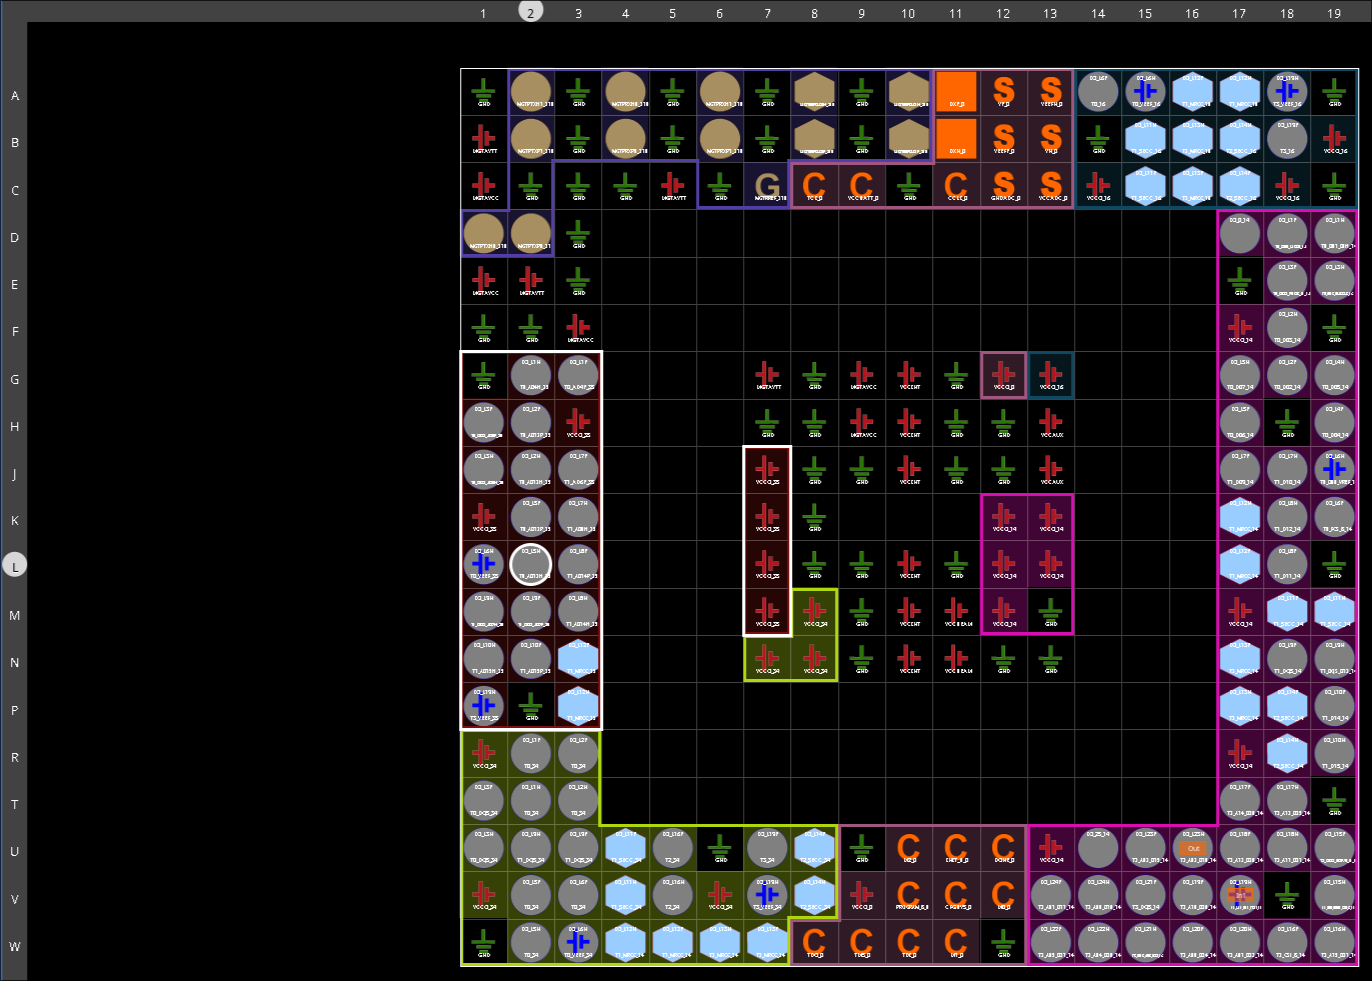
\includegraphics[width=0.5\textwidth]{Inverter-GATE-FLOOR-PLAN.png}
    \label{Inverter Gate, Floor Plan}
\end{figure}
\begin{figure}[!!htbpbp]
    \centering
    \caption{Inverter Gate Constraints}
    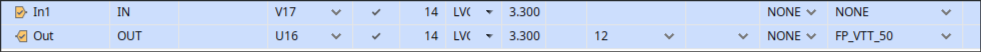
\includegraphics[width=0.75\textwidth]{Inverter-GATE-CONSTRAINTS.png}
    \label{Inverter Gate, Constrants}
\end{figure}\\
After this, I then ran the waveform simulation properly, as the circuit was properly implemented, as well as having the correct schematic. The waveform returned the following, as shown in Figure 33, as well as shown in Table 5 with its truth table.\\
\begin{figure}[!!htbpbp]
    \centering
    \caption{Inverter Gate Waveform}
    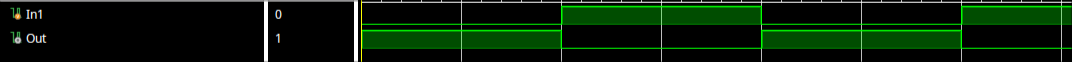
\includegraphics[width=0.75\textwidth]{Inverter-GATE-WAVEFORM.png}
    \label{Inverter Gate, Waveform}
\end{figure}\\
\begin{center}
    Truth Table 5: Inverter Gate Waveform
    \begin{displaymath}
    \begin{array}{|c|c|}
    In1 & \neg(In1)\\
    \hline
    F & T\\
    F & T\\
    T & F\\
    T & F\\
    \end{array}
    \end{displaymath}
\end{center}
The waveform here shows that the inverter simply turns the current state to the opposite type, for example from true to false and vice versa.
\newpage % 2 Input 5 Output
\subsection{2 Input 5 Output Gate}
Now to create the 2 Input, 5 Outputs gate, of which looks like the following, at its most basic form:\\
\begin{figure}[!!htbpbp]
    \centering
    \caption{2 Input, 5 Outputs Gate}
    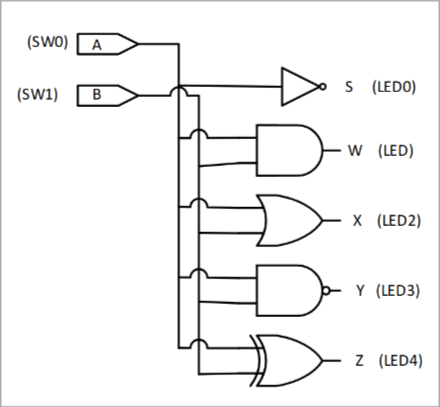
\includegraphics[width=0.5\textwidth]{2input-GATE.png}
    \label{2 Input 5 Output Gate, Simple}
\end{figure}\\
After inputting the following code for the Verilog module, of which is shown below in Figure 35, I then compiled the schematic to ensure that it is correctly modeled.\\
\begin{figure}[!!htbpbp]
    \centering
    \caption{Verilog Code for 2 Input, 5 Output Gate}
    \begin{verbatim}
    module 2_Input_5_Output(
        input A, B,
        output S, W, X, Y, Z
        );
        
        assign S = ~A;
        assign W = A & B;
        assign X = A | B;
        assign Y = ~(A & B);
        assign Z = A ^ B;
        
    endmodule
    \end{verbatim}
\end{figure}\\
And from that code it compiled this schematic (Figure 36) which has 2 inputs, being A and B, as well as 5 outputs, being S, W, X, Y, and Z. Alongside this, the device floor plan is shown as well, in Figure 37, as properly implemented according to the basic form shown in Figure 34, as well as the constraints for the simulation to take place (shown in Figure 38).\\
\begin{figure}[!!htbpbp]
    \centering
    \caption{2 Input, 5 Output Gate Schematic}
    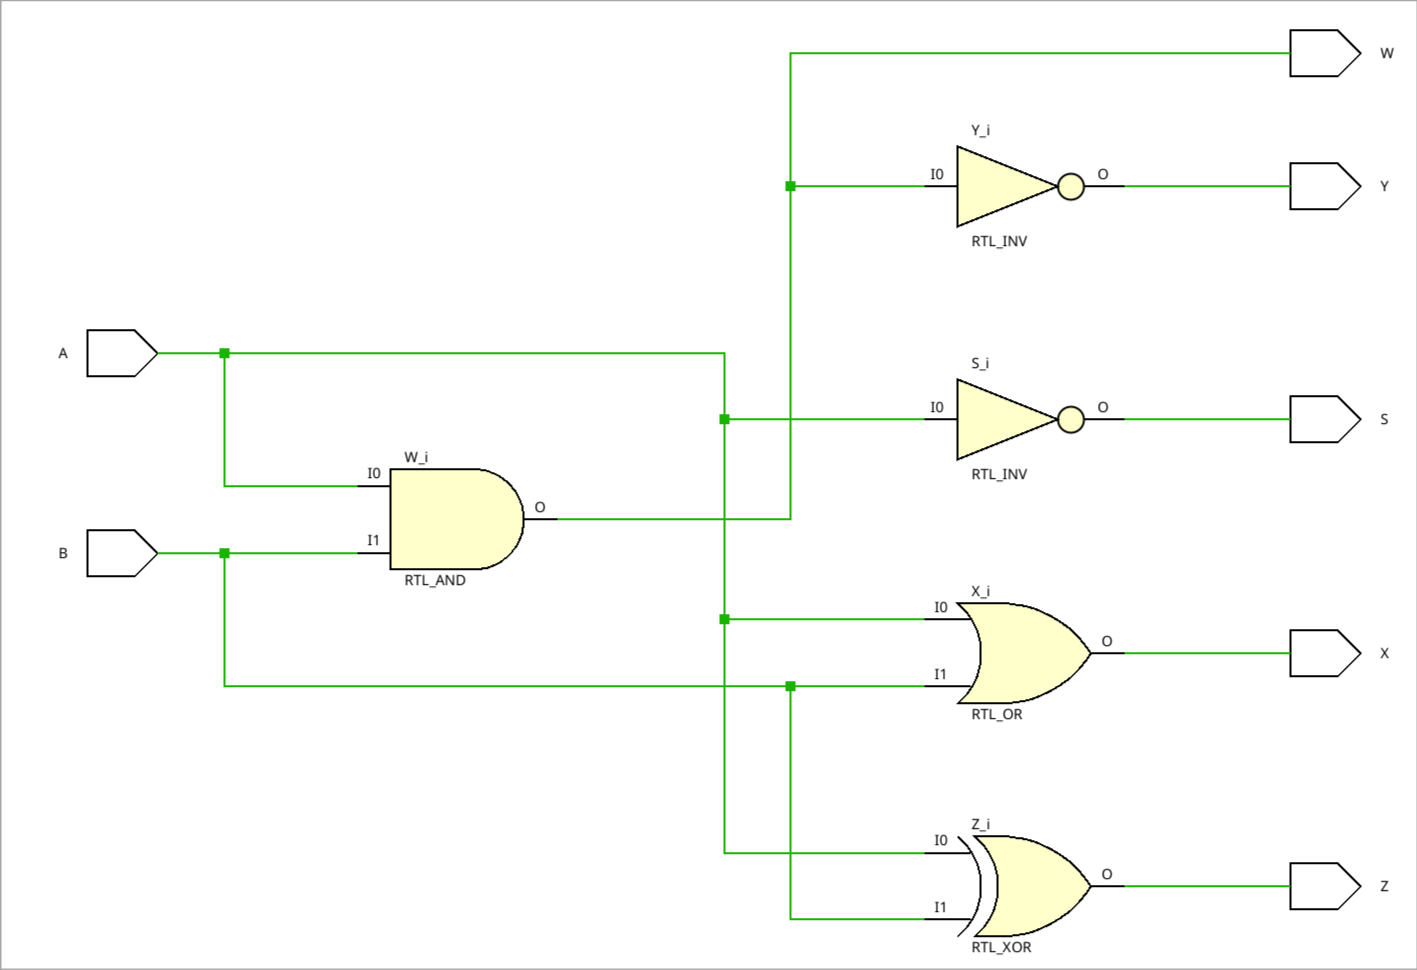
\includegraphics[width=0.5\textwidth]{2input-GATE-SCHEMATIC.png}
    \label{2 Input 5 Output, Schematic}
\end{figure}\\
\begin{figure}[!!htbpbp]
    \centering
    \caption{Inverter Gate Floor Plan}
    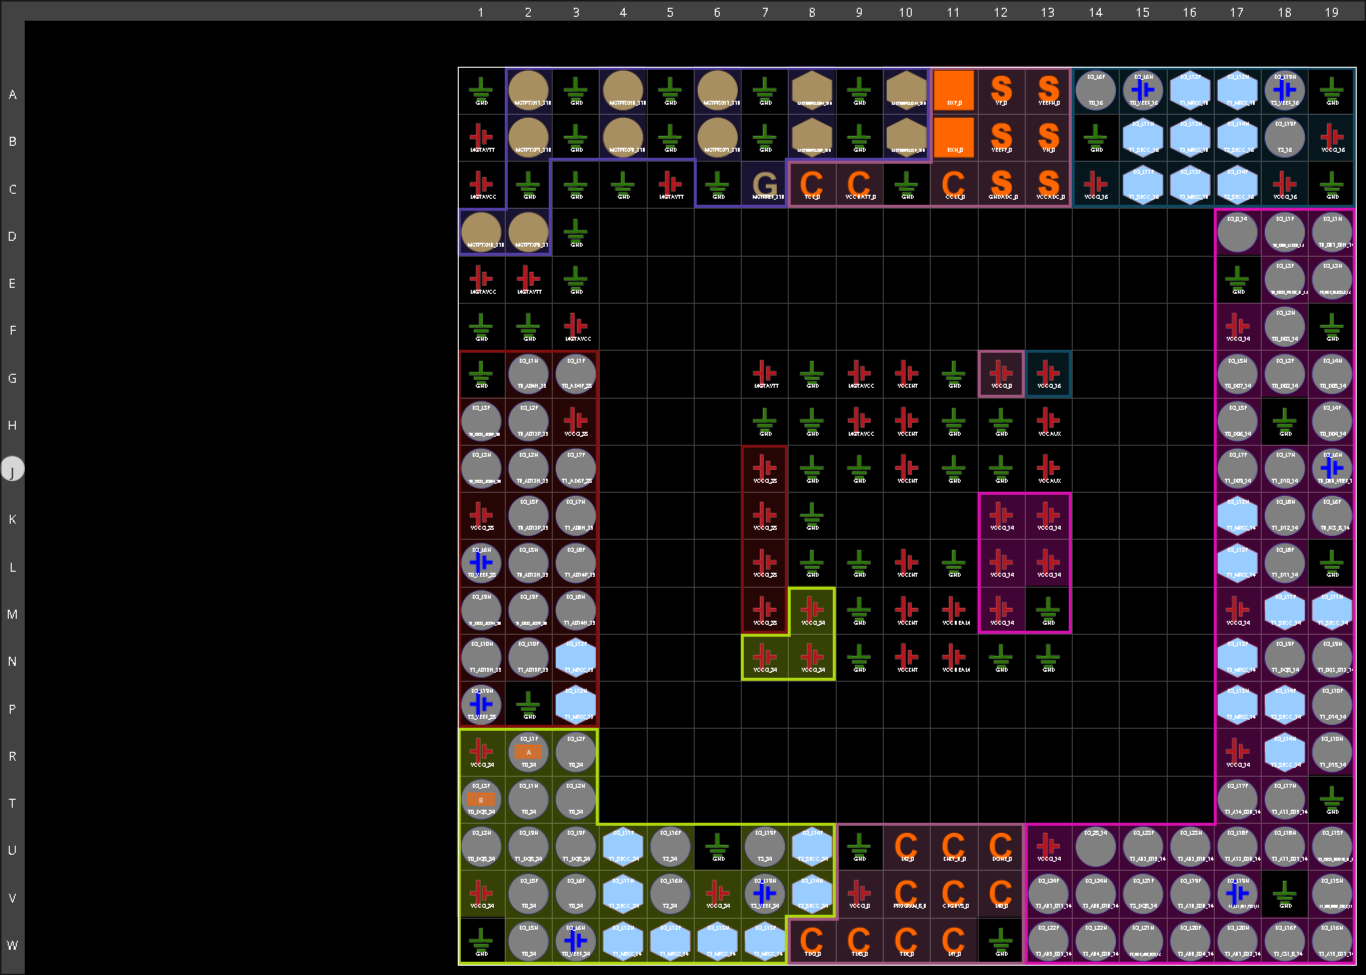
\includegraphics[width=0.5\textwidth]{2input-GATE-FLOOR-PLAN.png}
    \label{2 Input 5 Output, Floor Plan}
\end{figure}\\
\begin{figure}[!!htbpbp]
    \centering
    \caption{2 Input, 5 Output Gate Constraints}
    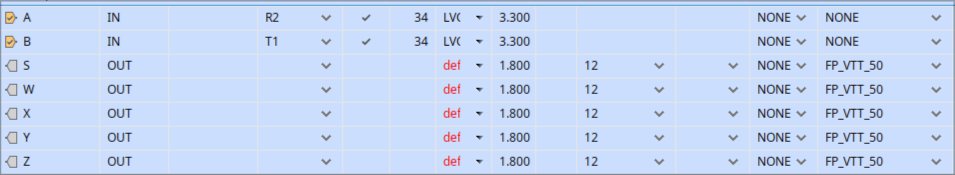
\includegraphics[width=0.75\textwidth]{2input-GATE-CONSTRAINTS.png}
    \label{2 Input 5 Output Gate, Constrants}
\end{figure}\\
After this, I then ran the waveform simulation properly, as the circuit was properly implemented, as well as having the correct schematic. The waveform returned the following, as shown in Figure 39, as well as shown in Table 6 with its truth table.\\
\begin{figure}[!!htbpbp]
    \centering
    \caption{2 Input, 5 Output Gate Waveform}
    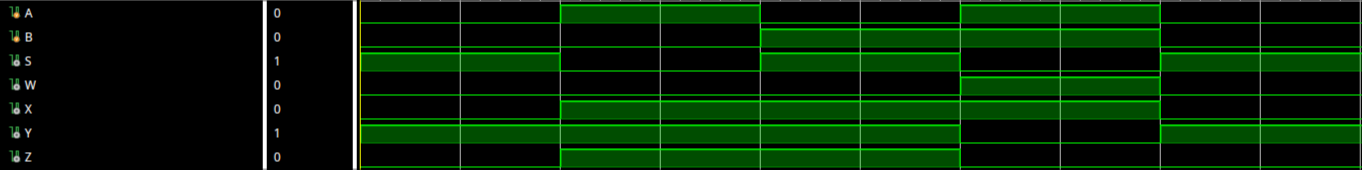
\includegraphics[width=0.75\textwidth]{2input-GATE-WAVEFORM.png}
    \label{2 Input 5 Output Gate, Waveform}
\end{figure}\\
\begin{center}
    Truth Table 6: 2 Input, 5 Output Gate Waveform
    \begin{displaymath}
    \begin{array}{|c c|c c c c c|}
    A & B & S & W & X & Y & Z\\
    \hline
    F & T & T & F & F & T & F\\
    F & T & T & F & T & T & T\\
    T & F & F & F & T & T & T\\
    T & F & F & T & T & F & F\\
    \end{array}
    \end{displaymath}
\end{center}
The waveform here is showing that all S does is simply INVERT the value of A, and is independent from the rest. W is simply an AND gate between the 2 inputs, and also is independent of the rest of the operations. X is an OR gate between the 2 inputs, and, again, is independent of the rest of the operations being done. Y is a NAND gate and, again, is independent of the rest of the operations. And Z is a XOR gate, and like the rest before it, is independent of the operations that go on in parallel with it.
\section{Test Steps}
The designs were tested by first running them through a simulation based off of a test bench (of which you see in the waveform figures in Section 4). Each input was set to cycle so that every single permutation was shown in the test bench. After testing, and proving correct from hand calculations, the design was then programmed onto the Basys 3 board, and all of the switches were then tested manually, so that they can be confirmed for a third time.
\section{Conclusion}
The entire experiment was a glaring success. The results were perfectly as expected, and all tests/checks agreed with one another harmoniously. Alongside this, the testing of the gate logic helped with my understanding of how they function as well as cemented them with the lab reports summarization.
\end{document}
